\documentclass[titlepage]{article}

\usepackage[margin=1in]{geometry}
\usepackage{csquotes}
\usepackage{fancyhdr}
\usepackage{marginnote}
\usepackage[style=apa]{biblatex}
\usepackage{enumitem}
\usepackage{scrextend}
\usepackage[bottom]{footmisc}
\usepackage{tikz}
\usepackage{amsmath,amssymb,amsbsy}
\usepackage{bm,physics}
\usepackage[hidelinks]{hyperref}
\usepackage{subfiles}

\MakeOuterQuote{"}

\fancypagestyle{main}{
    \fancyhf{}
    \fancyhead[L]{\leftmark}
    \fancyhead[R]{MATH 27000}
    \fancyfoot[R]{Labalme\ \thepage}
}
\fancypagestyle{plain}{
    \fancyhead{}
    \renewcommand{\headrulewidth}{0pt}
}

\reversemarginpar

\addbibresource{\subfix{../main.bib}}
\DefineBibliographyStrings{english}{bibliography={References}}

\setitemize[3]{label={\scriptsize$\blacksquare$}}

\deffootnotemark{\textsuperscript{\textup{[}\thefootnotemark\textup{]}}}
\deffootnote[1.8em]{0em}{0em}{\textsuperscript{\thefootnote}}

\colorlet{rex}{red!80!black!90!orange!80}

\DeclareMathOperator{\re}{Re}
\DeclareMathOperator{\im}{Im}
\DeclareMathOperator{\Hom}{Hom}

\newcommand{\R}{\mathbb{R}}
\newcommand{\C}{\mathbb{C}}
\newcommand{\D}{\mathbb{D}}
\newcommand{\Ss}{\mathbb{S}}
\newcommand{\Hh}{\mathbb{H}}

\numberwithin{equation}{section}

\title{
    MATH 27000 (Basic Complex Variables) Final Project\\
    Written Report
}
\author{Steven Labalme}

\begin{document}




\renewcommand{\thepage}{C}
\maketitle



\pagenumbering{roman}
\tableofcontents
\newpage



\pagenumbering{arabic}
\pagestyle{main}
\renewcommand{\leftmark}{Abstract}
\begin{center}
    \section*{Abstract}
    \addcontentsline{toc}{section}{Abstract}
\end{center}
The \textbf{time-independent Schr\"{o}dinger equation}, Equation \ref{eqn:Schrodinger1D} below, is an ordinary differential equation that physicists and chemists care about.
\begin{equation}\label{eqn:Schrodinger1D}
    -\frac{\hbar^2}{2m}\dv[2]{\psi(x)}{x}+V(x)\cdot\psi(x) = E\psi(x)
\end{equation}
This differential equation allows them to convert a `potential energy function' $V:\R\to\R$ of interest into a corresponding `wave function' $\psi:\R\to\R$. Some potential energy functions $V$ give rise to \textbf{special} differential equations, which are differential equations that occur often enough in the applied sciences to warrant special consideration, often expressed through extensive dedicated literature. Two such special differential equations are the \textbf{Hermite equation} and \textbf{Legendre equation}, Equations \ref{eqn:Hermite} and \ref{eqn:Legendre} below, respectively.
\begin{equation}\label{eqn:Hermite}
    \dv[2]{H}{x}-2x\dv{H}{x}+(\mu-1)H(x) = 0
\end{equation}
\begin{equation}\label{eqn:Legendre}
    (1-x^2)\dv[2]{P}{x}-2x\dv{P}{x}+\ell(\ell+1)P(x) = 0
\end{equation}
While the solutions to these equations and their properties are often discussed in undergraduate quantum mechanics courses for both physics and chemistry students, the derivations are not commonly given.\par
In Section \ref{sse:qmech}, we will situate the Hermite and Legendre equations within their context in quantum mechanics. We will first answer the age-old question, "what exactly \emph{is} quantum mechanics?" Then, we will introduce the Hermite equation as a problem whose theoretical solution enabled the creation of the microwave, and the Legendre equation as a problem whose theoretical solution provided chemists with the shapes of the atomic orbitals.\par
In Section \ref{sse:solving}, we will solve the Hermite and Legendre equations by using a chain of ansatzs and $u$-substitutions that culminate in a rewrite in the form of the \textbf{hypergeometric equation}, introduced in Problem Set 2 and restated below in Equation \ref{eqn:hypergeometricEq}.
\begin{equation}\label{eqn:hypergeometricEq}
    z(1-z)\dv[2]{u}{z}+[c-(a+b+1)z]\dv{u}{z}-abu = 0
\end{equation}
This equation can then be solved with the \textbf{hypergeometric function}, Equation \ref{eqn:hypergeometricF} below.
\begin{equation}\label{eqn:hypergeometricF}
    {}_2F_1(a,b;c;z) := \sum_{n=0}^\infty\frac{(a)_n(b)_n}{n!(c)_n}z^n
\end{equation}\par
Carrying out this procedure will leave us with computable solutions, but not with \emph{easily} computable solutions. To aid us in transforming the original solution into a more computationally friendly one, Section \ref{sse:complex} will reintroduce several topics in complex analysis presented throughout the quarter. These include the Cauchy integral formula and the residue theorem. Two additional topics that will be introduced are the \textbf{gamma function} and the \textbf{generating function}.\par
Lastly, in Section \ref{sse:applications}, we will apply these topics to derive \textbf{Rodrigues's formula} for the solutions to the Legendre equation, Equation \ref{eqn:Rodrigues} below, and a \textbf{recursion formula} for the solutions to the Hermite equation, Equation \ref{eqn:recursionHermite} below.
\begin{equation}\label{eqn:Rodrigues}
    P_\ell(x) = \frac{1}{2^\ell\ell!}\dv[\ell]{x}(x^2-1)^\ell
\end{equation}
\begin{equation}\label{eqn:recursionHermite}
    H_{n+1}(x) = 2xH_n(x)-2nH_{n-1}(x)
\end{equation}\par
The content of this paper was adapted from \textcite{bib:Seaborn} as well as my class notes for the University of Chicago's CHEM 26100 Quantum Mechanics and PHYS 23410 Quantum Mechanics I courses, \textcite{bib:CHEM26100Notes} and \textcite{bib:PHYS23410Notes}, respectively.
\newpage



\renewcommand{\leftmark}{\firstmark}
\renewcommand{\sectionmark}[1]{\markboth{Section \thesection\ (#1)}{}}
\renewcommand{\subsectionmark}[1]{}
\section{Introduction to Quantum Mechanics}\label{sse:qmech}
What follows is an intentionally brief, somewhat handwavey introduction to the broad discipline of quantum mechanics. In the name of being concise in my background, I will intentionally skip some details in a manner that might annoy a seasoned physics professor, but should provide a clear picture for anyone with minimal to no experience in the subject. Let's begin.


\subsection{Historical Development of Quantum Mechanics}
In classical physics, developed by Sir Isaac Newton in the 1600s, matter is thought of as being composed of particles whose motion is governed by Newton's laws, most famously, the following second-order differential equation.
\begin{equation}\label{eqn:Newton2nd}
    -\dv{V}{x} = F 
    = ma
    = m\dv[2]{x}{t}
\end{equation}
Practitioners of classical physics analyze larger objects as collections of particles, each of which evolves under Newton's laws. Simply put, matter is thought of as having a fundamentally \emph{particle-like} nature. This method of thinking about the universe stood unchallenged for 300 years and is still widely used today for applications ranging from building bridges to designing rocket ships.\par
However, modern physicists no longer accept classical physics as an \emph{everywhere applicable} model of the universe in which we live. In the early 1900s, experimentalists began to make observations of very small things. These observations called the universality of the postulates of classical physics into question. The most prominent example called into question the idea that matter is fundamentally particle-like. This example is described in the following paragraph.\par
The story begins with two of Einstein's 1905 \emph{annus mirabilis} papers, in particular those that culminated in the photoelectric effect and mass-energy equivalence equations (left and right below, respectively).
\begin{align*}
    E &= h\nu = \frac{hc}{\lambda}&
    E &= mc^2
\end{align*}
Combining these equations via transitivity yields the surprising result that light has mass! In particular, the mass $m$ of a beam of light is inversely proportional to its wavelength $\lambda$:
\begin{align*}
    mc^2 &= \frac{hc}{\lambda}\\
    m &= \frac{h}{\lambda c}\\
    m &\propto \frac{1}{\lambda}
\end{align*}
This may seem an absurd statement to one who has not worked extensively with quantum mechanics, but no matter how strange it may seem, it \emph{is} backed up by experimental evidence. Therefore, as scientists, we have to accept it until proven wrong. Almost two decades after this surprising discovery, a young doctoral student named Louis de Broglie was procrastinating his dissertation when he decided to turn in the following equation as the centerpiece of his four-page PhD thesis.
\begin{equation*}
    \lambda = \frac{h}{mc}
\end{equation*}
The Paris committee was ready to fail him, but they wrote to Einstein first. Fortunately for de Broglie, Einstein recognized the importance of this idea: That just like light has the matter-like property of mass, mass has the wave-like property of wavelength. Essentially, de Broglie had just postulated that fundamental particles of matter, such as electrons, have a wavelike nature. A few years later, the Davisson-Germer experiment --- an update to Thomas Young's double-slit experiment, famous for verifying the wavelike nature of light --- confirmed the wavelike nature of electrons. Once again, it may seem absurd to say that electrons can be both particles and waves, but this is what current experimental data suggests.\par
So what is matter? Newton said it's particles and provided plenty of evidence to substantiate that claim. De Broglie said it's waves and provided (or, rather, had others provide) plenty of evidence to substantiate this claim. Modern physicists and chemists will say that matter has a \textbf{dual wave-particle nature}. Essentially, this means that there are some experiments in which matter behaves like a particle and some in which it behaves like a wave; we will use each model when appropriate and leave the true nature of matter unsettled until we have more data.\par
So, if matter is a wave, then it is spread out over all space in some sense. It does not exist locally at some point $x$ (like a particle does), but rather at each point $x\in\R$, it should have some intensity $\psi(x)$ given by a \textbf{wave function} $\psi:\R\to\R$. A logical next question is whether or not there is an analogy to Newton's second law (Equation \ref{eqn:Newton2nd}), that is, a constraint we can put on the behavior and form of $\psi$. A year after de Broglie's breakthrough, Erwin Schr\"{o}dinger provided exactly such a constraint. While in the Swiss Alps with his mistress --- it wasn't only Oppenheimer! --- Schr\"{o}dinger postulated that in one dimension, $\psi$ should satisfy the time-independent Schr\"{o}dinger equation introduced in Equation \ref{eqn:Schrodinger1D} and restated below.
\begin{equation*}
    -\frac{\hbar^2}{2m}\dv[2]{\psi(x)}{x}+V(x)\cdot\psi(x) = E\psi(x)
\end{equation*}
At first glance, this appears to be a quite complicated and unmotivated postulate. In fact, it is. Theoretical physicist and renowned jokester Richard Feynman is quoted as having said, "where did we get that [equation] from? Nowhere. It is not possible to derive it from anything you know. It came from the mind of Schr\"{o}dinger." Feynman, true to character, was being mildly facetious, but the core of what he says is true: It was a pretty out-of-left-field result.\par
At this point, you (the reader) have all the necessary background to motivate quantum mechanics. The remainder of the subject consists of solving the Schr\"{o}dinger equation (and its generalizations) given potential energy functions $V$ "of interest," which is more mathematical than anything else. Two particular potential energy functions "of interest" are the harmonic oscillator potential (a parabola) and the central force field. We will discuss these two potentials and their applications more extensively in the following two sections.


\subsection{Motivating the Hermite Equation}
Think about popcorn. Think about how fluffy and buttery it is. Think about all the positive childhood memories you have of eating popcorn, be it at home, at the movies, or with friends. Am I making you hungry yet? Would you like to stop reading this and go throw a packet in the microwave? Well without quantum mechanics, you couldn't!\par
Microwaves work by shooting light of just the right frequency at your food so that molecules in it --- which are already vibrating harmonically --- vibrate faster. Faster vibrations means warmer food. But how do we know what frequency of light to use? How do we analyze the vibrating molecule we seek to irradiate?\par
One way of modeling a vibrating molecule is as a quantum harmonic oscillator, that is, a quantum particle subject to the following potential energy function.
\begin{equation*}
    V(x) = \frac{1}{2}kx^2
\end{equation*}
Sparing you the gory details, if we plug this potential energy function into the Schr\"{o}dinger equation and do some rearranging, we end up with the Hermite equation, introduced in Equation \ref{eqn:Hermite} and restated below.
\begin{equation*}
    \dv[2]{H}{x}-2x\dv{H}{x}+(\mu-1)H(x) = 0
\end{equation*}
To solve the Hermite equation, we need complex analysis and hypergeometric functions.


\subsection{Motivating the Legendre Equation}
Another place we can make use of quantum mechanics is in chemistry. Once atoms and molecules were discovered, chemistry developed as the discipline that uses atoms and molecules to "do stuff," be it synthesizing a new medicine, mass-producing the ammonia fertilizer that feeds the planet, and much more. "Doing stuff" with atoms and molecules, however, is greatly facilitated by a good understanding of how atoms and molecules interact, and hence how they're structured. Once again, quantum mechanics provides the answers we need.\par
A classic example is the electronic structure of the hydrogen atom, which consists of a single electron (a quantum particle) existing in the following potential. Note that the $e$ in the numerator is not Euler's number but rather is the charge of an electron.
\begin{equation*}
    V(r) = -\frac{e^2}{4\pi\varepsilon_0r}
\end{equation*}
Sparing you the gory details once again, if we plug this into the Schr\"{o}dinger equation and do some rearranging, we end up with the following precursor to the Legendre equation.
\begin{equation}\label{eqn:LegendreGenPre}
    (1-x^2)\dv[2]{P}{x}-2x\dv{P}{x}+\left[ \lambda-\frac{m^2}{1-x^2} \right]P(x) = 0
\end{equation}
Importantly, Equation \ref{eqn:LegendreGenPre} is \emph{not} the same as the Legendre equation, which is Equation \ref{eqn:Legendre}. Legendre's equation will actually only arise in the course of solving Equation \ref{eqn:LegendreGenPre}. Don't worry --- we'll get there.\par
Lastly, note that solving Equation \ref{eqn:LegendreGenPre} --- like solving Hermite's equation --- requires complex analysis and hypergeometric functions.
\newpage



\section{Solving the Hermite and Legendre Equations}\label{sse:solving}
\subsection{Mathematical Prerequisites}\label{sss:prereqs}
Standard coursework in calculus and differential equations --- along with this quarter's content on complex analysis --- almost entirely suffices to understand the following derivations. However, here are a few useful definitions as reminders, along with a couple of new ones.
\begin{definition}
    A \textbf{Pochhammer symbol} is an abbreviated notation for a constant derived from a given number $a$ in a particular way. It is defined inductively as follows, where $a\in\C$ and $n\in\N_0$, and is denoted by $\bm{(a)_n}$.
    \begin{align*}
        (a)_0 &:= 1\\
        (a)_n &:= a(a+1)(a+2)(a+3)\cdots(a+n-1)\tag{$n=1,2,3,\dots$}
    \end{align*}
\end{definition}
\begin{definition}\label{dfn:hypergeometricEqn}
    Let $a,b,c\in\C$ be constants independent of the complex variable $z$. Then the differential equation
    \begin{equation*}
        z(1-z)\dv[2]{u}{z}+[c-(a+b+1)z]\dv{u}{z}-abu = 0
    \end{equation*}
    is called the \textbf{hypergeometric equation}.
\end{definition}
\begin{definition}
    The \textbf{hypergeometric function} is a particular solution of the hypergeometric equation. It is denoted by $\bm{{}_2F_1(a,b;c;z)}$ and given by
    \begin{equation*}
        {}_2F_1(a,b;c;z) := \sum_{n=0}^\infty\frac{(a)_n(b)_n}{n!(c)_n}z^n
    \end{equation*}
\end{definition}
\begin{definition}\label{dfn:hypergeometricEqnC}
    Let $a,c\in\C$ be constants independent of the complex variable $z$. Then the differential equation
    \begin{equation*}
        z\dv[2]{u}{z}+(c-z)\dv{u}{z}-au = 0
    \end{equation*}
    is called the \textbf{confluent hypergeometric equation}. It is a particular restricted case of the hypergeometric equation introduced in Definition \ref{dfn:hypergeometricEqn}.
\end{definition}
\begin{definition}
    The \textbf{confluent hypergeometric function} is a particular solution of the confluent hypergeometric equation. It is denoted by $\bm{{}_1F_1(a;c;z)}$ and given by
    \begin{equation*}
        {}_1F_1(a;c;z) := \sum_{n=0}^\infty\frac{(a)_n}{n!(c)_n}z^n
    \end{equation*}
\end{definition}
To get more familiar with Pochhammer symbols (and introduce a result that will be useful in a later derivation), consider the function
\begin{equation*}
    f(z) = (1-z)^s
\end{equation*}
This function is analytic for any $s\in(-1,1)$. Using standard rules of differentiation, we can see that
\begin{align*}
    f'(z) &= -s(1-z)^{s-1}\\
    f''(z) &= (-1)^2s(s-1)(1-z)^{s-2}\\
    &\ \ \vdots\\
    f^{(k)}(z) &= (-1)^ks(s-1)\cdots(s-k+1)(1-z)^{s-k}\\
    &= (-1)^k(s)_k(1-z)^{s-k}\\
    &= (-s)_k(1-z)^{s-k}
\end{align*}
Thus, the Pochhammer symbol considerably simplifies the typically complicated expression for the $k^\text{th}$ derivatives of $(1-z)^s$. It follows that we can write the Taylor series for $(1-z)^s$ in a similarly simple form:
\begin{equation}\label{eqn:1zs}
    (1-z)^s = \sum_{k=0}^\infty\frac{(-s)_k}{k!}z^k
\end{equation}
Note that in converting $(-1)^k(s)_k$ to $(-s)_k$, we used a Pochhammer symbol identity! Here are some more, many of which will be useful in later derivations.
\begin{enumerate}
    \item \label{pci:1}$n!=(n-m)!(n-m+1)_m$.
    \item \label{pci:2}$(c-m+1)_m=(-1)^m(-c)_m$.
    \item \label{pci:3}$(n+m)!=n!(n+1)_m$.
    \item \label{pci:4}$n!=m!(m+1)_{n-m}$.
    \item \label{pci:5}$(2n-2m)!=2^{2n-2m}(n-m)!(\frac{1}{2})_{n-m}$.
    \item \label{pci:6}$(c)_{n+m}=(c)_n(c+n)_m$.
    \item \label{pci:7}$(c)_n=(-1)^m(c)_{n-m}(-c-n+1)_m$.
    \item \label{pci:8}$(c)_n=(-1)^{n-m}(c)_m(-c-n+1)_{n-m}$.
    \item \label{pci:9}$(-n)_{m-k}=(-n)_{m-n}(m-2n)_{n-k}$.
\end{enumerate}


\subsection{Hermite Equation}
We begin with Equation \ref{eqn:Hermite}, but with the independent variable denoted by $\rho$ instead of $x$:
\begin{equation*}
    \dv[2]{H}{\rho}-2\rho\dv{H}{\rho}+(\mu-1)H(\rho) = 0
\end{equation*}
We seek to rearrange this differential equation into the form of the confluent hypergeometric equation using variable changes. An \emph{independent} variable change is desirable here because it can alter the first two terms without affecting the zero-order term, which a comparison with Definition \ref{dfn:hypergeometricEqnC} will show is already in the right form.\par
Begin with the general modification $s:=\alpha\rho^n$, where $\alpha,n$ are parameters to be determined. Via the chain rule, the differential operators transform under this substitution into
\begin{align*}
    \dv{\rho} &= \dv{s}{\rho}\cdot\dv{s}\\
    &= n\alpha\rho^{n-1}\cdot\dv{s}\\
    &= n\alpha(\alpha^{-1/n}s^{1/n})^{n-1}\cdot\dv{s}\\
    &= n\alpha^{1/n}s^{1-1/n}\cdot\dv{s}
\end{align*}
and, without getting into the analogous gory details,
\begin{equation*}
    \dv[2]{\rho} = n^2\alpha^{2/n}s^{2-2/n}\dv[2]{s}+n(n-1)\alpha^{2/n}s^{1-2/n}\dv{s}
\end{equation*}
Now another thing that the confluent hypergeometric equation tells us is that the second-order term needs an $s$ in the coefficient. Thus, since $s^{2-2/n}$ is the current coefficient, we should choose $n=2$ so that $s^{2-2/2}=s^1=s$ is in the coefficient. This simplifies the operators to
\begin{align*}
    \dv{\rho} &= 2\alpha^{1/2}s^{1/2}\cdot\dv{s}&
    \dv[2]{\rho} &= 4\alpha s\dv[2]{s}+2\alpha\dv{s}
\end{align*}
and hence the differential equation to
\begin{align*}
    0 &= 4\alpha s\dv[2]{h}{s}+2\alpha\dv{h}{s}-2\cdot\alpha^{-1/2}s^{1/2}\cdot 2\alpha^{1/2}s^{1/2}\cdot\dv{h}{s}+(\mu-1)h(s)\\
    &= 4\alpha s\dv[2]{h}{s}+(2\alpha-4s)\dv{h}{s}+(\mu-1)h(s)\\
    &= \alpha s\dv[2]{h}{s}+\left( \frac{\alpha}{2}-s \right)\dv{h}{s}-\frac{1}{4}(1-\mu)h(s)
\end{align*}
Finally, to give the right coefficient in the second-order term and complete the transformation into the confluent hypergeometric equation, pick $\alpha=1$.
\begin{equation*}
    0 = s\dv[2]{h}{s}+\left( \frac{1}{2}-s \right)\dv{h}{s}-\frac{1}{4}(1-\mu)h(s)
\end{equation*}
At this point, solving with the hypergeometric function, along with some additional quantum mechanics and hypergeometric machinations\footnote{See my extended writeup in \textcite[23-25]{bib:FinalProject}.} leads to the final set of solutions
\begin{equation*}
    H_n(\rho) = \sum_{k=0}^{[n/2]}\frac{(-1)^kn!}{k!(n-2k)!}(2\rho)^{n-2k}
\end{equation*}
where $[x]$ is the \textbf{floor function}, which takes $x\in\R$ to the greatest integer less than or equal to $x$. Note also that $n$ is an index, and any nonnegative integer value of $n$ will lead to a usable solution to the Hermite equation.


\subsection{Legendre Equation}
Solving the Hermite equation was indicative of the techniques used to solve special differential equations and, apart from the choice of the form of the variable substitution $s=\alpha\rho^n$, was fairly well motivated. Solving Equation \ref{eqn:LegendreGenPre} uses many of the same techniques, but is far more involved, lengthy, and reliant on "because it works" mathematics. As such, I have relegated the details to my notes\footnote{See my writeup of the full solution in \textcite[27-34]{bib:FinalProject}.} and will present only a sketch here.\par
We begin with Equation \ref{eqn:LegendreGenPre}, but with the dependent variable denoted by $f$ instead of $P$:
\begin{equation*}
    (1-x^2)\dv[2]{f}{x}-2x\dv{f}{x}+\left[ \lambda-\frac{m^2}{1-x^2} \right]f(x) = 0
\end{equation*}\par
To start breaking down this equation, we use the (unmotivated) substitution
\begin{equation*}
    f(x) = v(x)w(x)
\end{equation*}
which gets us to
\begin{equation*}
    (1-x^2)vw''(x)+[2(1-x^2)v'-2xv]w'(x)+\left[ (1-x^2)v''-2xv'+\left( \lambda-\frac{m^2}{1-x^2} \right)v \right]w(x) = 0
\end{equation*}
For our next (unmotivated) substitution, we will let $v(x)=(1-x^2)^a$. To pin down the exact value of $a$, we employ a partially motivated constraint to get
\begin{equation*}
    v(x) = (1-x^2)^{\pm|m|/2}
\end{equation*}
Using this substitution gets us to
\begin{equation*}
    (1-x^2)w''(x)-2(1\pm|m|)xw'(x)-(m^2\pm|m|-\lambda)w(x) = 0
\end{equation*}
Lastly, we motivate and use the substitution
\begin{equation*}
    z = \frac{1}{2}(1-x)
\end{equation*}
which gets us to
\begin{equation*}
    z(1-z)w''(z)+[1\pm|m|-2(1\pm|m|)z]w'(z)-(m^2\pm|m|-\lambda)w(z) = 0
\end{equation*}
Using a little bit more algebra, we can fully transform the above into the form of the original hypergeometric equation and read off the solution as
\begin{equation*}
    w(z) = {}_2F_1(\underbrace{\tfrac{1}{2}(1-\sqrt{4\lambda+1})\pm|m|}_a,\underbrace{\tfrac{1}{2}(1+\sqrt{4\lambda+1})\pm|m|}_b;\underbrace{1\pm|m|}_c;z)
\end{equation*}
Employing an assumption from quantum mechanics that was left undiscussed in Section \ref{sse:qmech}, we choose the positive sign in every instance of the $\pm$ above. A further assumption from quantum mechanics allows us to solve for
\begin{equation*}
    \lambda = \ell(\ell+1)\tag{$\ell=0,1,2,\dots$}
\end{equation*}
and express the full and final set of solutions to Equation \ref{eqn:LegendreGenPre} as the following.
\begin{equation}\label{eqn:LegendreGenPreSolution}
    f_{\ell m}(x) = A_{\ell m}(1-x^2)^{|m|/2}\,{}_2F_1(-\ell+|m|,\ell+|m|+1;|m|+1;\tfrac{1}{2}(1-x))
\end{equation}
Note that $\ell$ and $m$ are constants subject to certain constraints that index the solutions, just like $n$ from the Hermite equation. Note also that $A_{\ell m}$ is a normalization constant, the full form of which can be determined with complex analysis covered in \textcite{bib:Seaborn} but beyond the scope of this paper.\par
Lastly, note that using the substitution $\lambda=\ell(\ell+1)$ and taking $m=0$ transforms Equation \ref{eqn:LegendreGenPre} into Legendre's equation (Equation \ref{eqn:Legendre}), which is solved by the similarly restricted case of Equation \ref{eqn:LegendreGenPreSolution}:
\begin{equation}\label{eqn:LegendreSolution}
    f_\ell(x) = {}_2F_1(-\ell,\ell+1;1;\tfrac{1}{2}(1-x))
\end{equation}
\newpage



\section{Relevant Topics in Complex Analysis}\label{sse:complex}
First, recall the Cauchy integral formula from the 4/2 lecture, restated as follows. Note that the closed curve $C$ must contain $z$.
\begin{equation*}
    f(z) = \frac{1}{2\pi i}\oint_C\frac{f(t)}{t-z}\dd{t}
\end{equation*}
Differentiating the Cauchy integral formula, we obtain the following result which will be used more than once in what follows.
\begin{equation*}
    f^{(n)}(z) = \frac{n!}{2\pi i}\oint_C\frac{f(t)}{(t-z)^{n+1}}\dd{t}
\end{equation*}\par
Additionally, we will state and prove a restricted version of the residue theorem. What follows is less general than what was presented in class on 5/2, but it is perfectly adequate for our purposes.
\begin{theorem}\label{trm:residue}
    If $C$ is a curve that encloses $N$ isolated singularities of $f$, the $k^\text{th}$ one being at $z_k$, then we have
    \begin{align*}
        \oint_Cf(z)\dd{z} &= \sum_{k=1}^N\oint_{C_k}f(z)\dd{z}
            = 2\pi i\sum_{k=1}^Na_{-1}(z_k)\\
        &= 2\pi i[\emph{sum of residues}]
    \end{align*}
    \begin{proof}
        For the sake of this argument, we will discuss a region with two holes/singularities, but the argument easily generalizes.
        \begin{figure}[H]
            \centering
            \begin{subfigure}[b]{0.4\linewidth}
                \centering
                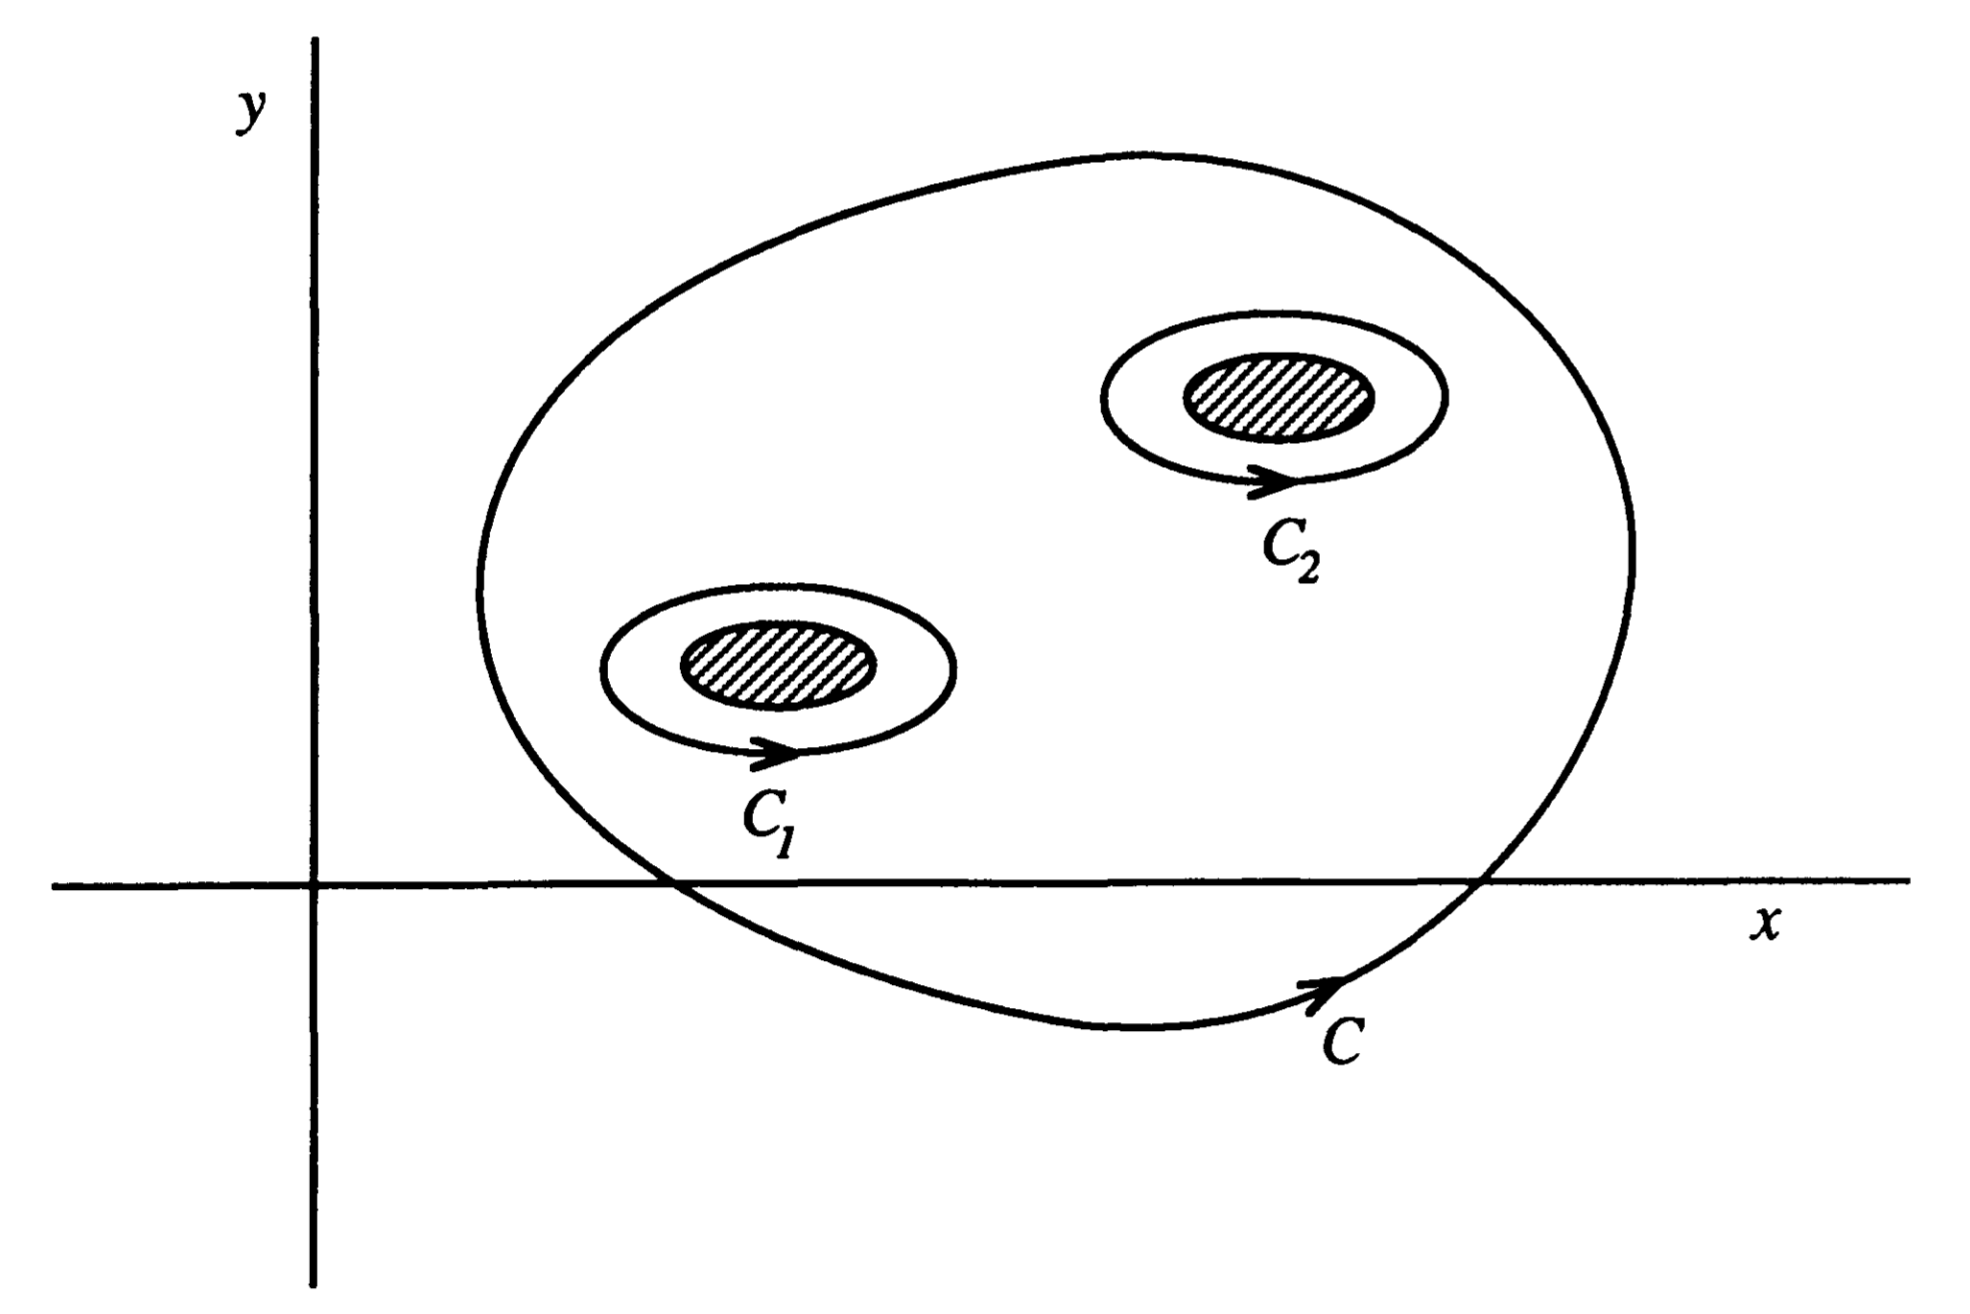
\includegraphics[width=0.9\linewidth]{residueTrma.png}
                \caption{Initial domain.}
                \label{fig:residueTrma}
            \end{subfigure}
            \begin{subfigure}[b]{0.4\linewidth}
                \centering
                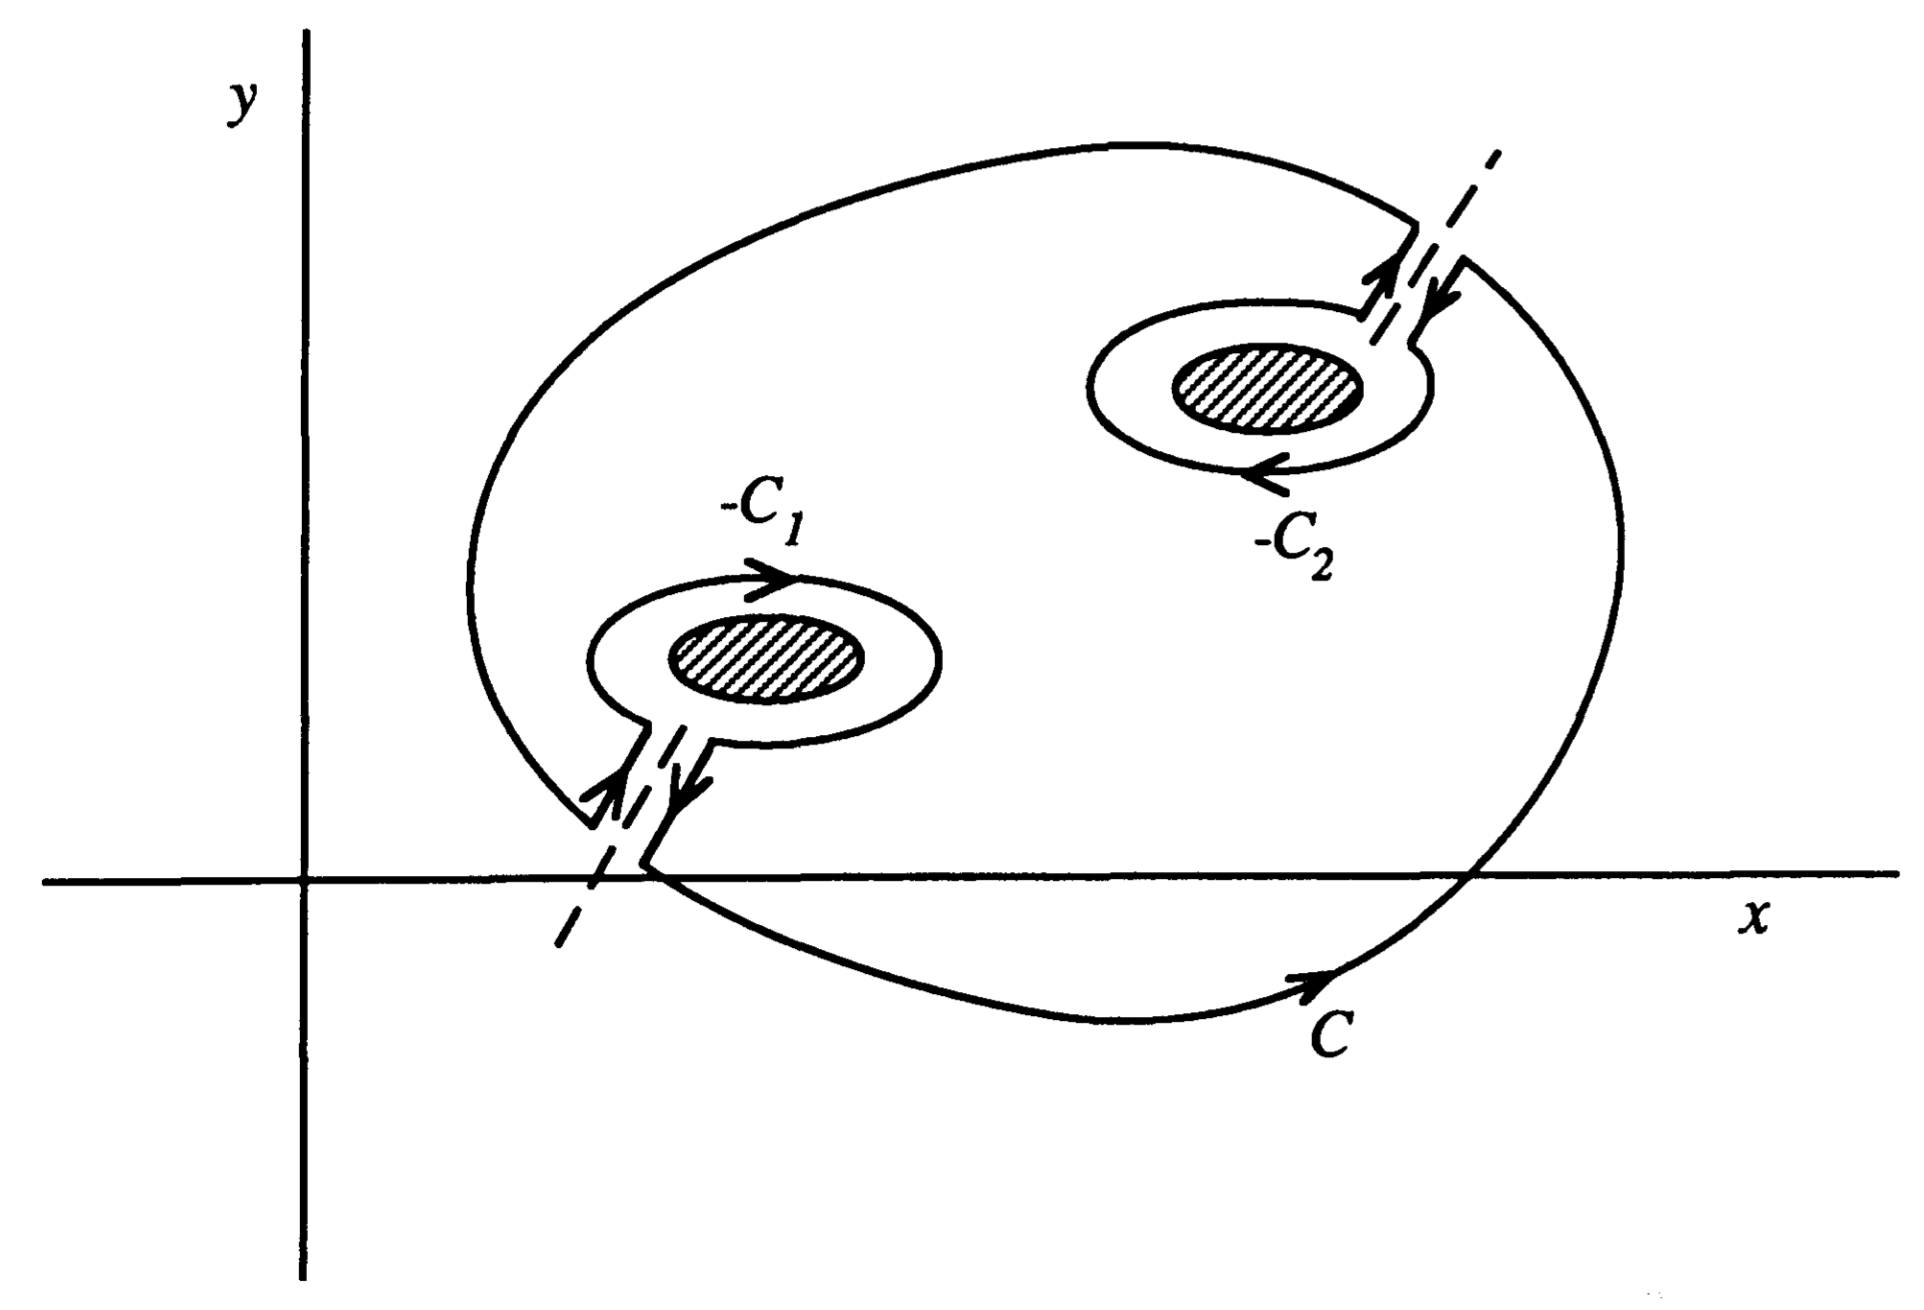
\includegraphics[width=0.9\linewidth]{residueTrmb.png}
                \caption{Cut lines.}
                \label{fig:residueTrmb}
            \end{subfigure}
            \caption{Proving the Cauchy Residue Theorem.\protect\footnotemark}
            \label{fig:residueTrm}
        \end{figure}
        \footnotetext{Pictures from \textcite[130]{bib:Seaborn}.}
        Draw curves $C_1,C_2$ around these holes/singularities oriented counterclockwise as well (Figure \ref{fig:residueTrma}). Make cut lines from $C$ to $C_1$ and from $C$ to $C_2$ (Figure \ref{fig:residueTrmb}). Thus, the single continuous contour
        \begin{equation*}
            C' := C+(-C_1)+(-C_2)+\text{cut lines}
        \end{equation*}
        encloses a simply connected region. Thus, by the definition of integrating over a multicurve,
        \begin{equation*}
            \oint_{C'}f(z)\dd{z} = \oint_Cf(z)\dd{z}+\oint_{-C_1}f(z)\dd{z}+\oint_{-C_2}f(z)\dd{z}
        \end{equation*}
        By the Cauchy integral theorem, the left-hand side of the above vanishes. Thus, rearranging, we obtain
        \begin{equation*}
            \oint_Cf(z)\dd{z} = \oint_{C_1}f(z)\dd{z}+\oint_{C_2}f(z)\dd{z}
        \end{equation*}
        At this point, we can evaluate each of the integrals on the RHS above via the definition of the residue to get the desired result.
    \end{proof}
\end{theorem}
Next, we will define a new mathematical object called the \textbf{gamma function}.
\begin{definition}
    The \textbf{gamma function} is an analytic continuation of the factorial function $!:\N\to\N$ to $\C$. It is denoted by $\bm{\Gamma(z)}$ and given by
    \begin{equation*}
        \Gamma(z) := \int_0^\infty t^{z-1}\e[-t]\dd{t}
    \end{equation*}
\end{definition}
The gamma function is most useful for its numerous properties, many of which are stated throughout \textcite{bib:Seaborn}. One that will be particularly useful for us is that the gamma function is a meromorphic function on $\C$, in particular one that is holomorphic everywhere except at the nonpositive integers, where it has simple poles (i.e., takes on $\infty\in\hat{\C}$). Another that will be useful is that $\Gamma(n+1)=n!$ for any $n\in\N_0$.\par
Lastly, we will define a new mathematical object called a \textbf{generating function}.
\begin{definition}
    The \textbf{exponential generating function} of an infinite sequence $\{p_n(x)\}$ of functions is a representation of that sequence as the $n^\text{th}$ derivatives of a formal power series in some variable indeterminate. We will denote the variable indeterminate by $t$ and the generating function by $g(x,t)$, giving us
    \begin{equation*}
        g(x,t) := \sum_{n=0}^\infty\frac{p_n(x)}{n!}t^n
    \end{equation*}
\end{definition}
\newpage



\section{Applications of Complex Analysis}\label{sse:applications}
\subsection{Deriving Rodrigues's Formula for the Legendre Polynomials}
In this section, we first convert Equation \ref{eqn:LegendreSolution} --- which is in the form of a hypergeometric series --- into another power series. This conversion will make use of some complex analysis! Then, for completion, we will finish converting this power series into Rodrigues's formula (Equation \ref{eqn:Rodrigues}), a neat little closed form expression for the Legendre polynomials. Note that throughout the following derivation, "Identity $n$" on the right side of the page refers to the invocation of the $n^\text{th}$ Pochhammer symbol identity from Section \ref{sss:prereqs}.

\subsubsection{An Alternate Power Series}
We begin from Equation \ref{eqn:LegendreSolution}, transcribed below with $n$ as an index instead of $\ell$:
\begin{equation*}
    P_n(x) = {}_2F_1(-n,n+1;1;\tfrac{1}{2}(1-x))
\end{equation*}
Using Equation \ref{eqn:1zs}, we can expand the above hypergeometric function to
\begin{align*}
    P_n(x) &= \sum_{k=0}^\infty\frac{(-n)_k(n+1)_k}{k!(1)_k2^k}(1-x)^k\\
    &= \sum_{k=0}^\infty\frac{(-n)_k(n+1)_k}{k!k!2^k}\sum_{m=0}^\infty\frac{(-k)_m}{m!}x^m\\
    &= \sum_{k=0}^\infty\frac{(-n)_k(n+1)_k}{k!k!2^k}\sum_{m=0}^\infty\frac{(k-m+1)_m}{m!}(-1)^mx^m\tag*{Identity \ref{pci:2}}
\end{align*}
Reverse the order of the sums, use some Pochhammer symbol identities, and use the fact that $(-n)_k=0$ for $k>n$ to get
\begin{align*}
    P_n(x) &= \sum_{m=0}^\infty\left( \sum_{k=0}^n\frac{(-n)_k(n+1)_k}{k!2^k}\frac{(k-m+1)_m}{k!} \right)\frac{(-1)^m}{m!}x^m\\
    &= \sum_{m=0}^\infty\left( \sum_{k=0}^n\frac{(-n)_k(n+1)_k}{k!2^k}\frac{1}{(k-m)!} \right)\frac{(-1)^m}{m!}x^m\tag*{Identity \ref{pci:1}}\\
    &= \sum_{m=0}^\infty\left( \sum_{k=0}^n\frac{(-n)_k(n+1)_k}{k!2^k}\frac{(k-m+1)_{n-k}}{(n-m)!} \right)\frac{(-1)^m}{m!}x^m\tag*{Identity \ref{pci:4}}\\
    &= \sum_{m=0}^\infty\left( \sum_{k=0}^n\frac{(-n)_k(n+1)_k}{k!2^k}\frac{(k-m+1)_{n-k}}{\Gamma(n-m+1)} \right)\frac{(-1)^m}{m!}x^m
\end{align*}
Since $\Gamma(n-m+1)$ diverges for $m>n$ (i.e., the nonnegative integers), it zeroes out all of those terms from its position in the denominator. Thus, we can rewrite the above double sum as
\begin{align*}
    P_n(x) &= \sum_{m=0}^n\frac{(-1)^mx^m}{m!\Gamma(n-m+1)}\sum_{k=0}^n\frac{(-n)_k(n+1)_k}{k!2^k}\frac{(k-m+1)_{n-k}}{1}\\
    &= \sum_{m=0}^n\frac{(-1)^mx^m}{m!\Gamma(n-m+1)}\sum_{k=0}^n\frac{(-1)^k(n-k+1)_k\cdot(n+1)_k}{k!2^k}\frac{(k-m+1)_{n-k}}{1}\tag*{Identity \ref{pci:2}}\\
    &= \sum_{m=0}^n\frac{(-1)^mx^m}{m!\Gamma(n-m+1)}\sum_{k=0}^n\frac{(-1)^k\cdot n!\cdot(n+1)_k}{k!2^k\cdot(n-k)!}\frac{(k-m+1)_{n-k}}{1}\tag*{Identity \ref{pci:1}}\\
    &= \sum_{m=0}^n\frac{(-1)^mx^mn!}{m!\Gamma(n-m+1)}\sum_{k=0}^n\frac{(-1)^k(n+1)_k}{k!2^k}\frac{(k-m+1)_{n-k}}{(n-k)!}\\
    &= \sum_{m=0}^n\frac{(-1)^mx^mn!}{m!\Gamma(n-m+1)}\sum_{k=0}^n\frac{(-n-1-k+1)_k}{k!2^k}\frac{(k-m+1)_{n-k}}{(n-k)!}\tag*{Identity \ref{pci:2}}
\end{align*}
Now observe that the sum on the right above kind of looks like the coefficient of the $n^\text{th}$ term in a Cauchy product expansion. We will use this observation and some complex analysis to rewrite said sum in a much simpler closed form.\par
In fact, with a little rewrite, we can put the above sum in exactly the form of the $n^\text{th}$ term in a Cauchy product expansion:
\begin{equation*}
    c_n = \sum_{k=0}^n\frac{(-n-1-k+1)_k}{k!2^k}\frac{(n-m-(n-k)+1)_k}{(n-k)!}
\end{equation*}
A logical next question to ask is, "what functions $u(t),v(t)$ would have such a coefficient in their Cauchy product $w(t)=u(t)v(t)$?" By the definition of the Cauchy product and Equation \ref{eqn:1zs}, it would have to be the functions
\begin{align*}
    u(t) &= \sum_{k=0}^\infty\frac{(-n-1-k+1)_k}{k!2^k}t^k&
        v(t) &= \sum_{k=0}^\infty\frac{(n-m-k+1)_k}{k!}t^k\\
    &= \sum_{k=0}^\infty\frac{(-1)^k(n+1)_k}{k!2^k}t^k&
        &= \sum_{k=0}^\infty\frac{(-1)^k(-n+m)_k}{k!}t^k\tag*{Identity \ref{pci:2}}\\
    &= \sum_{k=0}^\infty\frac{(n+1)_k}{k!}(-\tfrac{t}{2})^k&
        &= \sum_{k=0}^\infty\frac{(-n+m)_k}{k!}(-t)^k\\
    &= \left( 1+\frac{t}{2} \right)^{-n-1}&
        &= (1+t)^{n-m}
\end{align*}
Consequently,
\begin{equation*}
    w(t) = \left( 1+\frac{t}{2} \right)^{-n-1}(1+t)^{n-m}
\end{equation*}
Since $u,v$ were both analytic (as power series), $w$ must be analytic as well with
\begin{equation*}
    w(t) = \sum_{k=0}^\infty c_kt^k
\end{equation*}
Thus, by the formula for the derivative of the Cauchy integral formula, we know that the power series expansion of $w$ about 0 (a computationally nice point where $w$ is analytic) is the following, where $C$ is a closed curve encircling 0 but none of $w$'s singularities.
\begin{equation*}
    w(t) = \sum_{k=0}^\infty\left( \frac{1}{2\pi i}\oint_C\frac{w(\tau)}{\tau^{k+1}}\dd\tau \right)t^k
\end{equation*}
It follows that in particular,
\begin{align*}
    c_n &= \frac{1}{2\pi i}\oint_C\frac{w(t)}{t^{n+1}}\dd{t}\\
    &= \frac{1}{2\pi i}\oint_C\frac{(1+t)^{n-m}}{\left( 1+\tfrac{t}{2} \right)^{n+1}t^{n+1}}\dd{t}\\
    &= \frac{2^{n+1}}{2\pi i}\oint_C\frac{(1+t)^{n-m}}{(2t+t^2)^{n+1}}\dd{t}
\end{align*}
Now perform a $u$-substitution with $u:=2t+t^2$:
\begin{align*}
    c_n &= \frac{2^{n+1}}{2\pi i}\oint_C\frac{(1+t)^{n-m}}{u^{n+1}}\cdot\frac{\dd{u}}{2+2t}\\
    &= \frac{2^n}{2\pi i}\oint_C\frac{(1+t)^{n-m-1}}{u^{n+1}}\dd{u}\\
    &= \frac{2^n}{2\pi i}\oint_C\frac{[(1+t)^2]^{(n-m-1)/2}}{u^{n+1}}\dd{u}\\
    &= \frac{2^n}{2\pi i}\oint_C\frac{(1+2t+t^2)^{(n-m-1)/2}}{u^{n+1}}\dd{u}\\
    &= \frac{2^n}{2\pi i}\oint_C\frac{(1+u)^{(n-m-1)/2}}{u^{n+1}}\dd{u}
\end{align*}
Using Equation \ref{eqn:1zs}, we can transform the numerator of the integrand as follows.
\begin{align*}
    c_n &= \frac{2^n}{2\pi i}\oint_C\frac{1}{u^{n+1}}\sum_{r=0}^\infty\frac{(-\tfrac{n-m-1}{2})_r}{r!}(-u)^r\dd{u}\\
    &= \frac{2^n}{2\pi i}\oint_C\sum_{r=0}^\infty\frac{(-1)^r(\tfrac{n-m-1}{2}-r+1)_r}{r!}\frac{(-1)^ru^r}{u^{n+1}}\dd{u}\tag*{Identity \ref{pci:2}}\\
    &= \frac{2^n}{2\pi i}\sum_{r=0}^\infty\frac{(\tfrac{n-m-1}{2}-r+1)_r}{r!}\oint_Cu^{r-n-1}\dd{u}
\end{align*}
Since $C$ surrounds $t=0$ by definition, it also naturally surrounds $u=2(0)+(0)^2=0$. Thus, we may use the two definitions of the residue and Theorem \ref{trm:residue} to learn that
\begin{align*}
    c_n &= \frac{2^n}{2\pi i}\sum_{r=0}^\infty\frac{(\tfrac{n-m-1}{2}-r+1)_r}{r!}\cdot 2\pi i\res_0\left( \frac{1}{u^{n+1-r}} \right)\\
    &= 2^n\sum_{r=0}^\infty\frac{(\tfrac{n-m-1}{2}-r+1)_r}{r!}\res_0\left( \frac{1}{u^{n+1-r}} \right)
\end{align*}
Clearly, the "$a_{-1}$ term" of $u^{r-n-1}$ is only nonzero when $r=n$, and in this case, $a_{-1}=1$. Thus, we may neglect all terms in the above sum save the $r=n$ term, leaving us with
\begin{align*}
    c_n &= \frac{2^n(\tfrac{n-m-1}{2}-n+1)_n}{n!}\\
    &= \frac{2^n\left( -\tfrac{1}{2}(n+m-1) \right)_n}{n!}
\end{align*}
This is the final form to which we will simplify the original sum, and the derivation was greatly facilitated via the use of complex analysis.\par
Having simplified $c_n$, we can substitute it back into the expression for $P_n(x)$, obtaining
\begin{equation*}
    P_n(x) = \sum_{m=0}^n\frac{(-1)^mx^m2^n\left( -\tfrac{1}{2}(n+m-1) \right)_n}{m!(n-m)!}
\end{equation*}
Since the summation index $m\leq n$,\footnote{We neither stated nor proved this mathematical quirk of quantum mechanics in our derivation of the Legendre polynomials, but a statement and proof can be found in \textcite[32]{bib:FinalProject}.} we have that $\tfrac{1}{2}(n+m-1)<n$. Thus, $(-\tfrac{1}{2}(n+m-1))_n$ will reach zero (and hence be zero) whenever $n+m-1$ is an even integer, zeroing out those terms in the above summation. As such, we may define a new summation index $k$ by $2k:=n-m$; this one will only index over the nonzero terms of the above sum by keeping $n+m-1$ equal to an odd integer. Reindexing, we get
\begin{equation*}
    P_n(x) = \sum_{k=0}^{[n/2]}\frac{(-1)^{n-2k}x^{n-2k}2^n\left( k-n+\tfrac{1}{2} \right)_n}{(n-2k)!(2k)!}
\end{equation*}
Finally, use some more Pochhammer symbol identities to rewrite the expression above fully in terms of factorials.
\begin{equation*}
    P_n(x) = \sum_{k=0}^{[n/2]}\frac{(-1)^k(2n-2k)!}{2^nk!(n-k)!(n-2k)!}x^{n-2k}
\end{equation*}

\subsubsection{The Rodrigues Formula}
Looking at the above expression for $P_n(x)$, observe that the right two factorials and variable are actually, by definition, an $n^\text{th}$ derivative. Thus, we can make the substitution
\begin{equation*}
    P_n(x) = \sum_{k=0}^{[n/2]}\frac{(-1)^k}{2^nk!(n-k)!}\dv[n]{x}x^{2n-2k}
\end{equation*}
Let's investigate this $n^\text{th}$ derivative a bit more. Computationally, we have
\begin{equation*}
    \dv[n]{x}x^{2n-2k} = (n-2k+1)_nx^{n-2k}
\end{equation*}
Observe that like the analogous case in the previous derivation, $(n-2k+1)_n=0$ for $k\geq[\tfrac{n}{2}]+1$. Thus, we may formally add terms in the range $[\tfrac{n}{2}]+1\leq k\leq n$ to the sum without changing the value, resulting in
\begin{equation*}
    P_n(x) = \sum_{k=0}^n\frac{(-1)^k}{2^nk!(n-k)!}\dv[n]{x}x^{2n-2k}
\end{equation*}
Now reindex with $p=n-k$:
\begin{equation*}
    P_n(x) = \sum_{p=0}^n\frac{(-1)^{n-p}}{2^n(n-p)!p!}\dv[n]{x}x^{2p}
\end{equation*}
Consequently, we may rewrite the expression and compress it via a binomial expansion into the final form, matching Equation \ref{eqn:Rodrigues} up to the notational change $\ell\to n$.
\begin{align*}
    P_n(x) &= \frac{1}{2^nn!}\dv[n]{x}\sum_{p=0}^n\frac{n!}{p!(n-p)!}(x^2)^p(-1)^{n-p}\\
    &= \frac{1}{2^nn!}\dv[n]{x}(x^2-1)^n
\end{align*}


\subsection{Deriving a Recursion Formula for the Hermite Polynomials}
To derive the recursion formula, we will first derive a generating function for the Hermite polynomials. This generating function will allow us to easily represent the Hermite polynomials as a complex contour integral. Finally, from this representation, we will be able to derive the recursion formula. Let's begin.

\subsubsection{A Generating Function}
Postulate the existence of a generating function $g$ for the Hermite polynomials, and assume $g$ is analytic at and near $t=0$.\footnote{There is no reason that this must be true, but we are free to assume it and see where it gets us. If it gets us somewhere, we're golden!} Then
\begin{equation*}
    H_n(x) = \eval{\pdv[n]{t}g(x,t)}_{t=0}
\end{equation*}
Additionally, \textcite{bib:Seaborn} derived a Rodrigues-type formula for the Hermite polynomials, stated below, that will now be useful.
\begin{equation*}
    H_n(x) = (-1)^n\e[x^2]\dv[n]{x}\e[-x^2]
\end{equation*}
The above two equations can be combined by transitivity, yielding the following. This is the equation we will solve for $g$.
\begin{equation*}
    (-1)^n\e[x^2]\dv[n]{x}\e[-x^2] = \eval{\pdv[n]{t}g(x,t)}_{t=0}
\end{equation*}
Comparing the two sides, the following ansatz appears promising, where $f$ is another undetermined function.
\begin{equation*}
    g(x,t) = \e[x^2]f(x-t)
\end{equation*}
Using this, we obtain
\begin{equation*}
    \eval{\pdv[n]{t}g(x,t)}_{t=0} = \eval{\e[x^2]\pdv[n]{t}f(x-t)}_{t=0}
    = \eval{(-1)^n\e[x^2]\dv[n]{u}f(u)}_{t=0}
\end{equation*}
It follows by comparison with the Rodrigues formula for $H_n(x)$ that
\begin{equation*}
    f(u) = \e[-u^2]
\end{equation*}
Therefore, returning the substitution, we have that
\begin{equation*}
    g(x,t) = \e[x^2]\e[-(x-t)^2] = \sum_{n=0}^\infty\frac{H_n(x)}{n!}t^n
\end{equation*}

\subsubsection{A Contour Integral Representation}
Using the formula for the derivative of the Cauchy integral formula, another formula for the Taylor series of $g$ about $t=0$ is
\begin{equation*}
    g(x,t) = \sum_{n=0}^\infty\frac{g^{(n)}(x,t)}{n!}t^n
    = \sum_{n=0}^\infty\pdv[n]{t}g(x,t)\frac{t^n}{n!}
    = \sum_{n=0}^\infty\left( \frac{n!}{2\pi i}\oint_C\frac{g(x,t)}{t^{n+1}}\dd{t} \right)\frac{t^n}{n!}
\end{equation*}
where $C\ni 0$. Thus, by comparing this to the generating function, we learn that
\begin{equation*}
    H_n(x) = \frac{n!}{2\pi i}\oint_C\frac{g(x,t)}{t^{n+1}}\dd{t}
    = \frac{n!}{2\pi i}\oint_C\frac{\e[x^2]\e[-(x-t)^2]}{t^{n+1}}\dd{t}
    = \frac{n!}{2\pi i}\oint_C\frac{\e[2xt-t^2]}{t^{n+1}}\dd{t}
\end{equation*}

\subsubsection{The Recursion Formula}
We have that
\begin{equation*}
    H_n'(x) = \frac{n!}{2\pi i}\oint_C\frac{2t\e[2xt-t^2]}{t^{n+1}}\dd{t}
    = 2n\cdot \frac{(n-1)!}{2\pi i}\oint_C\frac{\e[2xt-t^2]}{t^{(n-1)+1}}\dd{t}
    = 2nH_{n-1}(x)
\end{equation*}
Differentiating both sides of the above (and using the above), we obtain
\begin{equation*}
    H_n''(x) = 2n\cdot H_{n-1}'(x)
    = 2n\cdot 2(n-1)H_{n-2}(x)
    = 4n(n-1)H_{n-2}(x)
\end{equation*}
Now recall that Hermite's equation reads
\begin{equation*}
    H_n''(x)-2xH_n'(x)+2nH_n(x) = 0
\end{equation*}
Thus, with our new definitions for $H_n'(x),H_n''(x)$, we obtain
\begin{align*}
    4n(n-1)H_{n-2}(x)-2x\cdot 2nH_{n-1}(x)+2nH_n(x) &= 0\\
    2(n-1)H_{n-2}(x)-2xH_{n-1}(x)+H_n(x) &= 0\\
    H_n(x) &= 2xH_{n-1}(x)-2(n-1)H_{n-2}(x)
\end{align*}
Redefining the indices $n-1\to n$ in the above yields the final recursion formula
\begin{equation*}
    H_{n+1}(x) = 2xH_n(x)-2nH_{n-1}(x)
\end{equation*}
in agreement with Equation \ref{eqn:recursionHermite}.
\newpage



\section{Discussion}
In this paper, we have motivated, stated, and derived several results concerning the Hermite and Legendre equations.\par
We began by situating these two equations within their context in quantum mechanics. Historically, we discussed what exactly quantum mechanics is and how it came to prominence. It then followed that it can be applied to a wide variety of everyday situations, including the creation of the microwave and a proper description of the atom. These two problems in particular were cited as the quantum mechanical origin of the Hermite and Legendre equations. In the following section, we solved these two equations using hypergeometric functions. After that, we introduced some topics from complex analysis and used these topics to rework our solutions into more convenient forms.\par
In total, we considered five forms of the solutions to the Hermite and Legendre equations: Polynomial series, generating functions, contour integral representations, recursion formulas, and Rodrigues-type fomulas. Each has its own merits and demerits. For example, the recursion formula is simple to use for small $n$, but takes more work at large $n$. Rodrigues-type formulas are quite compact, but require computing derivatives. Contour integrals are useful theoretically, but not practically computable. And so on.\par
A first-time or casual reader of this paper should leave with an appreciation of three main things: Quantum mechanics \emph{unconventionally} but \emph{accurately} predicts the behavior of the microworld; introductory \emph{calculus} and \emph{algebra} are enough to furnish many of its results; and complex analysis is an \emph{essential tool} to cast results in their \emph{simplest, most elegant, and most useful forms}.

\newpage



\renewcommand{\leftmark}{References}
\printbibliography[heading=bibintoc]




\end{document}